%%%%%%%%%%%%%%%%%%%%%%%%%%%%%%%%%%%%%%%%%
% a0poster Portrait Poster
% LaTeX Template
% Version 1.0 (22/06/13)
%
% The a0poster class was created by:
% Gerlinde Kettl and Matthias Weiser (tex@kettl.de)
% 
% This template has been downloaded from:
% http://www.LaTeXTemplates.com
%
% License:
% CC BY-NC-SA 3.0 (http://creativecommons.org/licenses/by-nc-sa/3.0/)
%
%%%%%%%%%%%%%%%%%%%%%%%%%%%%%%%%%%%%%%%%%

%----------------------------------------------------------------------------------------
%	PACKAGES AND OTHER DOCUMENT CONFIGURATIONS
%----------------------------------------------------------------------------------------

\documentclass[a0,portrait]{a0poster}

\usepackage{multicol} % This is so we can have multiple columns of text side-by-side
\columnsep=100pt % This is the amount of white space between the columns in the poster
\columnseprule=3pt % This is the thickness of the black line between the columns in the poster

\usepackage[svgnames]{xcolor} % Specify colors by their 'svgnames', for a full list of all colors available see here: http://www.latextemplates.com/svgnames-colors

\usepackage[sc]{mathpazo}
\linespread{1.08}         % Palatino needs more leading (space between lines)

\usepackage{graphicx} % Required for including images
\graphicspath{{figures/}} % Location of the graphics files
\usepackage{booktabs} % Top and bottom rules for table
\usepackage[font=normalsize,labelfont=sc]{caption} % Required for specifying captions to tables and figures
\usepackage{amsfonts, amsmath, amsthm, amssymb} % For math fonts, symbols and environments
\usepackage{wrapfig} % Allows wrapping text around tables and figures
\usepackage[utf8]{inputenc} 
\usepackage[detect-all]{siunitx}
\usepackage[T1]{fontenc}
\usepackage{titling}
\usepackage{authblk}
\usepackage{enumitem}
\usepackage[sc]{titlesec}

\setdescription{leftmargin=\parindent,labelindent=4\parindent}

\pretitle{\veryHuge \color{NavyBlue}}
\preauthor{\huge}
\postauthor{\par \vspace{2cm}
    \Large\texttt{matteo.abis@psi.ch}}
\newcommand{\subtitle}[1]{%
  \posttitle{%
    \par
    \color{Black}
    \Huge\textit{#1}
    \vspace{2cm}
    \par
    }%
}

\renewcommand\Affilfont{\Large}
\renewcommand{\labelitemi}{$\vcenter{\hbox{\tiny$\bullet$}}$}
\newenvironment{spacedcenter}{\vspace{2cm}\begin{center}}
        {\end{center}\vspace{2cm}\par}

\setlength{\parindent}{0cm}

\DeclareSIUnit{\voltpeak}{Vp}
\newcommand{\G}[1]{\ensuremath{G_{#1}}}
\newcommand{\energy}{\ensuremath{\mathcal{E}}}
\newcommand{\de}[1]{\ensuremath{\operatorname{d}\!{#1}}}


\begin{document}

\title{Optimization of X-ray grating interferometry}
\subtitle{and results on a \SI{160}{\kilo\voltpeak} lab source}
\author[1,2]{T. Th\"uring}
\author[1,2]{M. Abis}
\author[1,2]{M. Stampanoni}
\affil[1]{Institut für Biomedizinische Technik, ETH Z\"urich}
\affil[2]{Paul Scherrer Institut}
\date{}

%----------------------------------------------------------------------------------------
%	POSTER HEADER 
%----------------------------------------------------------------------------------------

% The header is divided into two boxes:
% The first is 75% wide and houses the title, subtitle, names, university/organization and contact information
% The second is 25% wide and houses a logo for your university/organization or a photo of you
% The widths of these boxes can be easily edited to accommodate your content as you see fit

\begin{minipage}[b]{0.75\linewidth}
    \maketitle
\end{minipage}
%
\begin{minipage}[b]{0.25\linewidth}
    
\includegraphics[width=15cm]{psi_logo.jpg}\\[2cm]
    
\includegraphics[width=15cm]{eth-logo.jpg}\\
\end{minipage}

\vspace{1cm} % A bit of extra whitespace between the header and poster content

%----------------------------------------------------------------------------------------

\begin{multicols}{2} % This is how many columns your poster will be broken into, a portrait poster is generally split into 2 columns

%----------------------------------------------------------------------------------------
%	INTRODUCTION
%----------------------------------------------------------------------------------------

\color{Navy} % SaddleBrown color for the introduction

\thispagestyle{empty}
\section*{Introduction}
Grating interferometry \cite{David2002} can perform phase-contrast imaging on
    conventional X-ray sources \cite{Pfeiffer2006}. This technique is sensitive to attenuation,
    refraction and scattering of the radiation.
    Analytical formulas are derived for the smallest detectable refraction
    angle and for the polychromatic visibility of the interference pattern
    as a function of the design parameters.
    Imaging at energies above \SI{100}{\kilo\eV}
    is particularly relevant for medical computed tomography and material
    science.
    Two Talbot-Lau interferometers were realized with 
    a design energy of \SI{100}{\kilo\eV} and
    \SI{120}{\kilo\eV}.

%----------------------------------------------------------------------------------------
%	OBJECTIVES
%----------------------------------------------------------------------------------------

\color{DarkSlateGray} % DarkSlateGray color for the rest of the content

\section*{Sensitivity of Talbot-Lau interferometers}
The sensitivity of a Talbot-Lau interferometer, or the smallest detectable
angle of refraction\cite{Modregger2011} is
\begin{equation*}
    \sigma_\alpha \propto \frac{p_2}{d}\frac{1}{v\sqrt{N}}
\end{equation*}
where $p_2$ is the period of the absorption grating \G{2}, $d$ is the
distance between \G{1} and \G{2}, $v$ is the visibility and $N$ is the
number of photons on the detector.

This suggests using an increased distance $d$ with setups at higher Talbot
orders, but this would also decrease the flux $N$. A sensitivity dependent
on the exposure time $t$ and the total setup length $s$ can be written as
\begin{align*}
    \frac{p_2}{d} &= \frac{p_0 + p_2}{s}\\
    N &\propto \frac{t}{s^2}\\
    \sigma_\alpha &\propto \frac{p_0 + p_2}{v\sqrt{t}}
\end{align*}

Therefore, the best sensitivity is achieved for smallest $p_0$ and
$p_2$. Since the period is generally limited by the fabrication technique,
where
the requirements for the two absorption gratings are the same, a
symmetric setup with $p_0 = p_2$ is the best combination.
%------------------------------------------------

\section*{Polychromatic visibility}
The visibility for the case of a polychromatic source can also be derived
analytically\cite{Thuering2014}. For each energy $\energy$ and a Talbot order $m \in
\{1,3,5,\ldots\}$, the visibility is
\begin{equation*}
    v(\energy) = \frac{2}{\pi} \left \lvert \sin^\eta \Big( \pi
    \frac{\energy_0}{\energy} \Big) \sin \Big( m \pi
    \frac{\energy_0}{\energy} \Big) \right \rvert
\end{equation*}
With $\energy_0$ the design energy, and $\eta = 2$ for a $\pi$-shifting beam splitter, and $\eta=1$ for a
$\pi / 2$ shift.
The total visibility can be calculated if the spectrum $\rho(\energy)$ is
known
\begin{equation*}
    v = \int v(\energy) \rho(\energy) \de \energy
\end{equation*}
This can be used to show the difference between a $\pi$ and a $\pi / 2$
shift in the \G{1} grating. The result is that the $\pi / 2$ has a
marginally better spectral acceptance only at the first Talbot order, and is
worse otherwise.

\begin{center}
    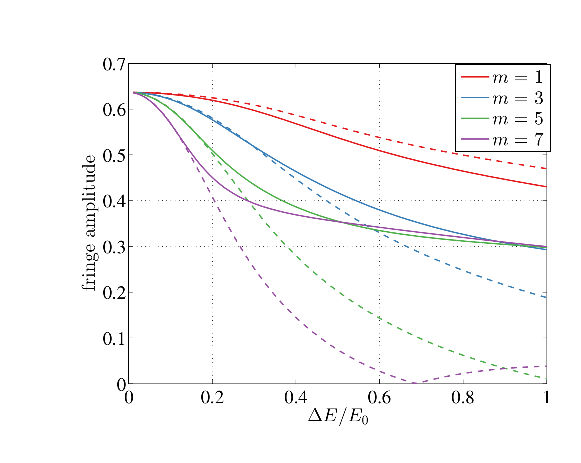
\includegraphics[width=0.5\linewidth]{polychromatic.eps}
    \captionof{figure}{Fringe visibility for a polychromatic beam of a point source as
    a function of the normalized energy bandwidth $\Delta E / E_0$ of a
gaussian spectrum for different talbot orders $m$ and for $\eta = 1$
(dashed lines) corresponding to a $\pi / 2$ shift in the phase grating
structures, compared to a $\pi$-shifting phase grating (solid lines).}
\end{center}

%----------------------------------------------------------------------------------------
%	ACKNOWLEDGEMENTS
%----------------------------------------------------------------------------------------
\section*{Acknowledgements}
We thank Gordan Mikuljan and István Mohácsi from PSI for the
work on the mechanical design and the SEM images
respectively, Joachim Schulz and Marco Walter from
Microworks GmbH, Germany, for the competent support on grating design
issues, Christian Kottler and Vincent Revol from Centre Suisse
d'Electronique et de Microtechnique (CSEM), Switzerland for the fruitful
discussions on the design of the system. This work has been partially
supported by the Competence Centre for Materials Science and Technology
(CCMX) of the ETH-Board, Project Nr. 61 and by the ERC Grant ERC-2012-StG 310005-PhaseX.
%----------------------------------------------------------------------------------------

\section*{Grating design}
The fabrication of gratings for X-ray energies above \SI{100}{\kilo\eV} is a
severe technical challenge. The requirement of an extreme aspect ratio is
overcome here with the idea of edge-on illumination.
The parameters for the two interferometers were chosen according to the
above principles: they are operated at the first Talbot order $m=1$, $d = p
/ 8 \lambda_0$ on a symmetric arrangement with $\pi$-shifting beam
splitters.
The gratings were manufactured by Microworks GmbH, Germany. The absorption gratings have a thickness of \SI{800}{\micro\metre}.
All gratings have a pitch $p$ of \SI{2.8}{\micro\metre}.
The interferometers are operated at the first Lohmann distance 
\begin{spacedcenter}
\begin{tabular}{lll}
    \textbf{design energy} & \SI{100}{\kilo\eV} & \SI{120}{\kilo\eV}\\
    \textbf{intergrating distance} & \SI{15.8}{\centi\metre} &
    \SI{18.9}{\centi\metre}\\
    \textbf{total length} & \SI{54}{\centi\metre} & \SI{61}{\centi\metre}\\
    \textbf{beam splitter} & gold & nickel \\
\end{tabular}
\end{spacedcenter}
\begin{center}
    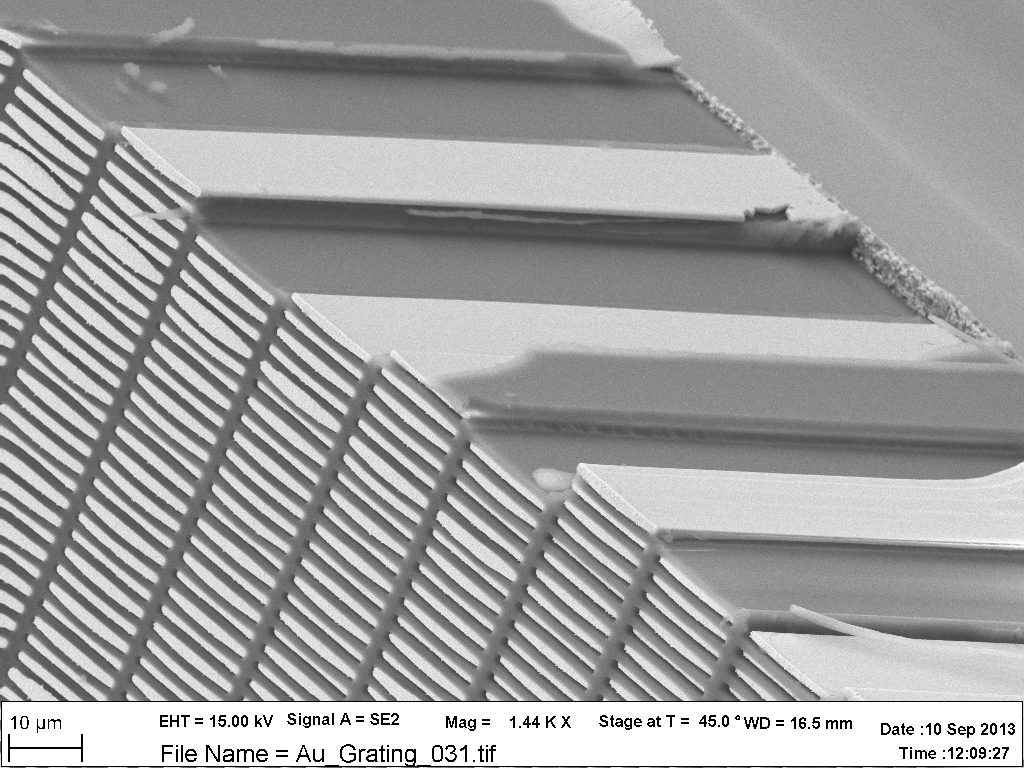
\includegraphics[width=0.5\linewidth]{Au_Grating_031.pdf}
    \captionof{figure}{scanning electron microscope image of the grating structures.}
\end{center}
%\columnbreak


%----------------------------------------------------------------------------------------
%	RESULTS 
%----------------------------------------------------------------------------------------

\section*{Experimental results}
The setups have a rather low average
visibility ($\sim\SI{6}{\percent}$) caused by the low quality of the
gratings. The first images show the three complementary contrasts retrieved
from the phase-stepping procedure \cite{Weitkamp2005}. 
\begin{spacedcenter}
    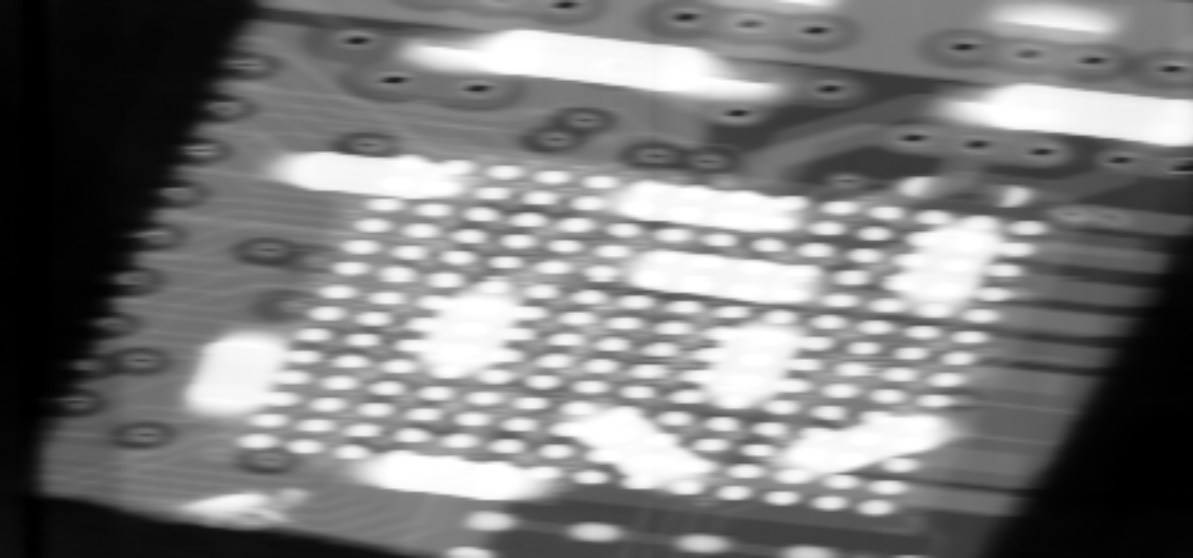
\includegraphics[width=0.3\linewidth,height=8cm]{images_S00075_S00071-img0.png}
    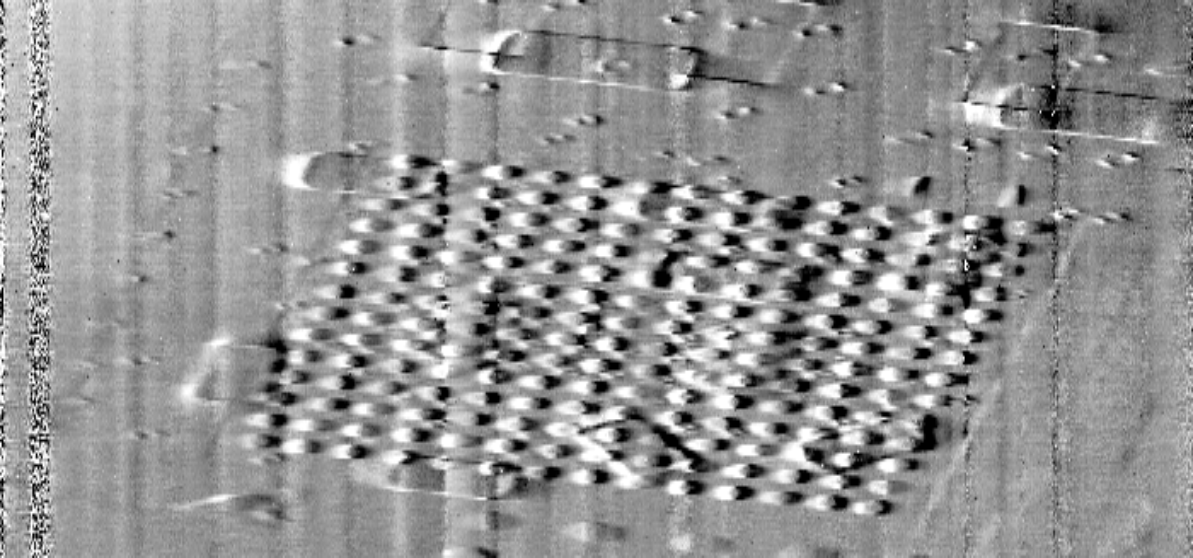
\includegraphics[width=0.3\linewidth,height=8cm]{images_S00075_S00071-img1.png}
    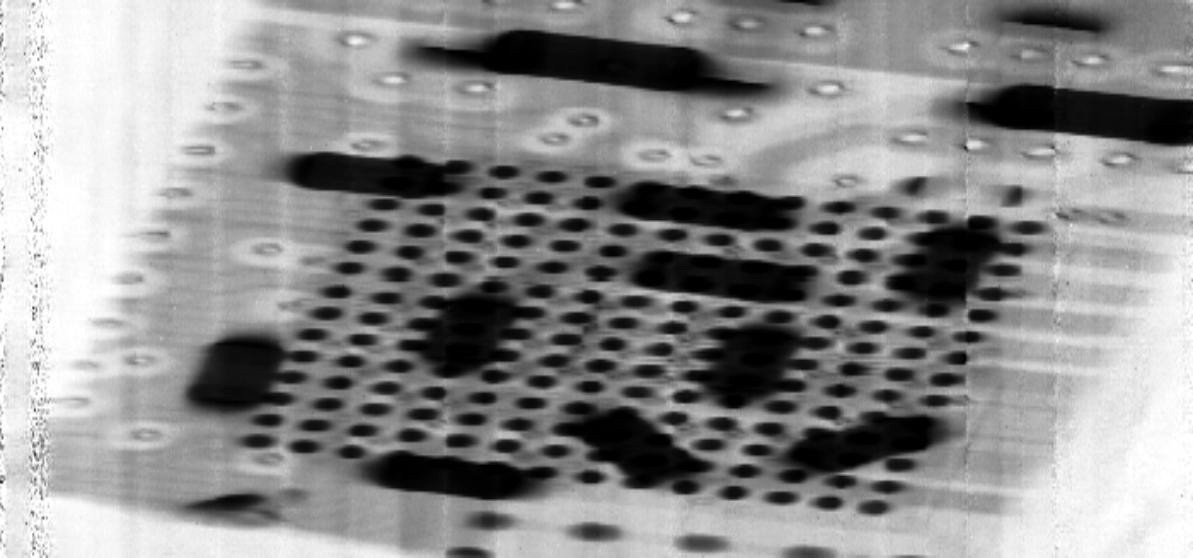
\includegraphics[width=0.3\linewidth,height=8cm]{images_S00075_S00071-img2.png}
    \captionof{figure}{Absorption, differential phase and dark-field image
        of a metal chip scanned in \SI{100}{\micro\m} steps. Field of view
        $\SI{2}{\centi\metre}\times\SI{2}{\centi\metre}$. \SI{100}{\kilo\eV}
    setup.}
\end{spacedcenter}
The exposure time has to be very long (\num{24} phase steps $\times$
\SI{15}{\second} per line) in order to reduce the noise given by the low visibility.

\color{DarkSlateGray} % Set the color back to DarkSlateGray for the rest of the content
 %----------------------------------------------------------------------------------------
%	REFERENCES
%----------------------------------------------------------------------------------------

\bibliographystyle{ieeetr} % Plain referencing style
\bibliography{library} % Use the example bibliography file sample.bib

\end{multicols}
\end{document}
